% !TeX root = ../thuthesis-example.tex
\externaldocument{chap05}
\chapter{紧耦合地图定位}

本章主要对紧耦合地图定位模块进行介绍。紧耦合定位的第一个关键过程是粗到细定位,本章中对选择这一过程的原因及如何实施进行了详细的介绍。此外,由于视觉惯性里程计和粗到细定位的坐标系不一致,无法直接使用,因此本章引入转换矩阵初始化和有效性检验两个步骤进行对齐。在此之后,紧耦合优化是定位的另一个关键过程,本章对这一过程进行了理论说明和公式推导,并以非线性优化技术完成实际优化。最后为了解决视觉惯性里程计的漂移问题,本章提出了转换矩阵更新过程,并对其进行了详细的介绍。

\section{整体设计}

紧耦合地图定位是整个定位系统的核心部分,其主要使用离线建图模块的多层次先验地图和视觉惯性里程计的相对位姿估计结果来计算相机在全局坐标系中的精确位姿,整体设计如图~\ref{fig:localization} 所示。

\begin{figure}
  \centering
  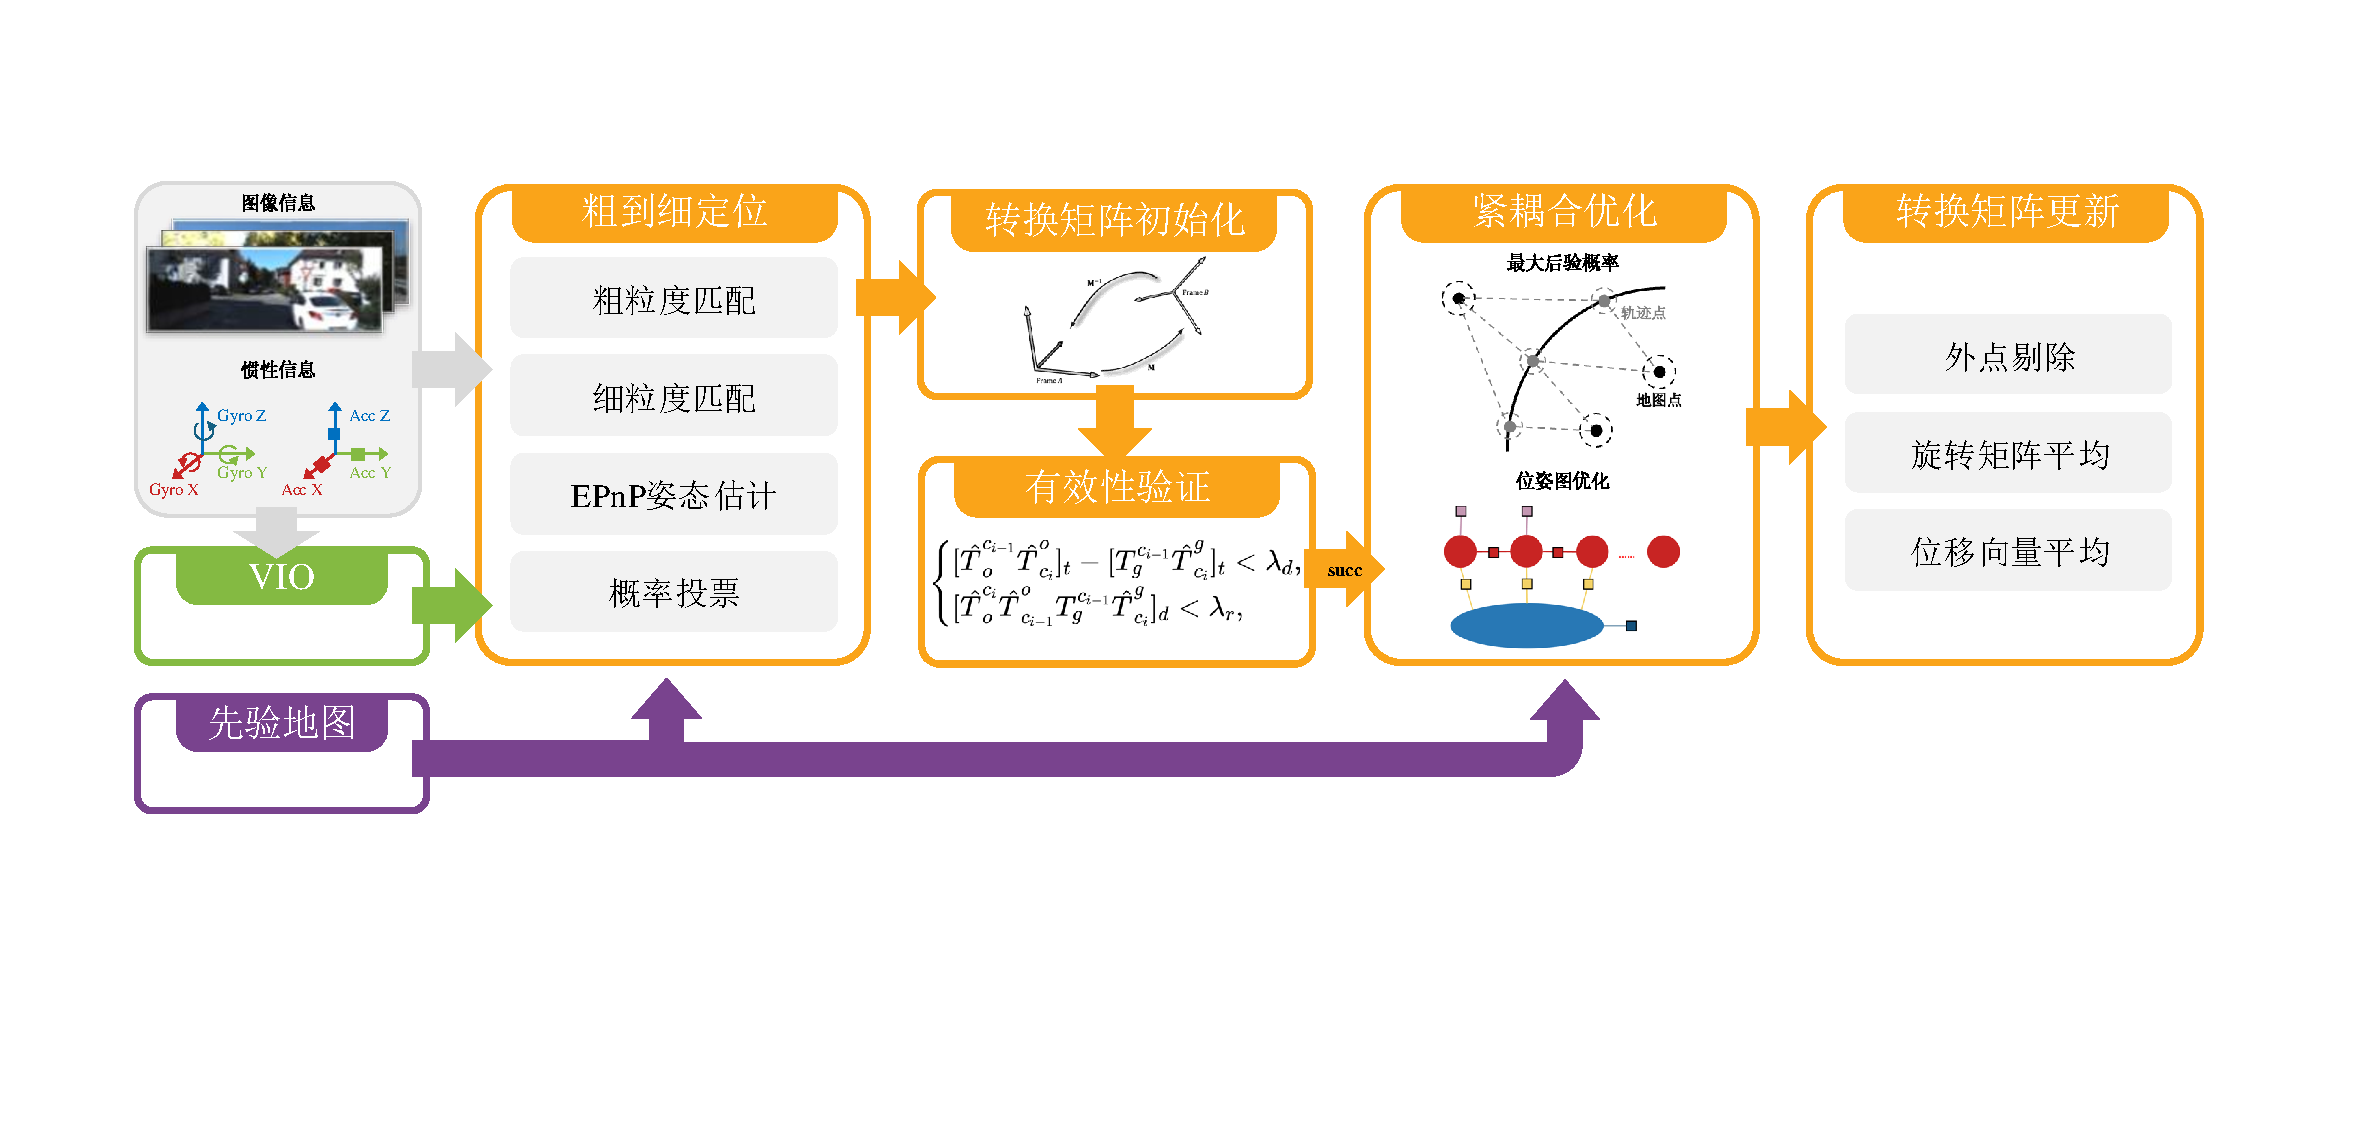
\includegraphics[width=1.0\linewidth]{localization.pdf}
  \caption{粗到细匹配过程}
  \label{fig:localization}
\end{figure}

整个模块的第一步是粗到细定位,其主要根据当前的图像观测和地图信息进行对比以及关联,从而获得相机在全局坐标系中的定位观测。粗到细匹配是粗到细定位的关键,其含义是首先根据粗粒度的图像级特征匹配结果和先验位置信息来获得图像的粗略位置范围,然后根据细粒度的像素级特征匹配结果来计算更精确的位姿结果。

除了粗到细定位,视觉惯性里程计同样可以获得位置观测结果,但是这两种定位方式的结果却因为分属全局坐标系$(\cdot)^{g}$和VIO世界坐标系$(\cdot)^{o}$而无法直接对齐。因此需要一个转换矩阵初始化过程来获得两个坐标系的对齐参数,即转换矩阵$\symbf{T}_o^{g}$。此外,由于转换矩阵对于整个定位过程有着重要作用,所以系统中对其成功有着严格要求,即只有当粗到细定位成功时,才会进入后续阶段。

在获得了两个坐标系的转换矩阵之后,理论上可以直接使用粗到细定位结果和转换后的视觉惯性里程计结果进行融合,但是考虑到粗到细定位结果可能会因为误匹配等原因而存在较大误差,因此需要使用有效性验证过程来判断粗到细定位结果的可靠性。如果粗到细定位的结果通过了检验,则优先选择其作为后续优化的初始值;否则,则需要使用经过转换的视觉惯性里程计结果作为初始位姿来进行后续优化。

为了获得较为精细的相机位姿,还需要进行紧耦合优化。这一步主要使用非线性优化的方法,将前面步骤中生成的粗到细定位结果、视觉惯性里程计输出以及先验地图的点云结构,以非线性优化的形式进行融合。在融合过程中考虑到地图本身所携带的误差,将先验地图的地图点视作服从高斯分布的概率点云,通过最大后验概率来求解相机位姿。

经过上述步骤后已经输出相机位姿,但是由于视觉惯性里程计自身在运行期间会产生漂移的累积,因此在经过长时间的运行后,视觉惯性里程计的世界坐标系已经产生了变化。如果此时依旧沿用之前的转换矩阵,则会导致视觉惯性里程计的误差传导到整个定位系统,因此转换矩阵的更新是有必要的。


\section{粗到细定位}
\label{sec:c2f_loc}

粗到细特征匹配是粗到细定位的核心步骤,粗到细匹配基于粗粒度和细粒度特征描述子,即图像描述符和点描述符。以往手工设计的特征描述子 \cite{lowe2004distinctive, rublee2011orb}和词袋模型是图像描述子和特征点描述子的常见选择,在这种形式下,所有关键帧的特征点描述子被聚类,聚类中心被汇总成一个词袋,新图像的特征点首先被分配到其最近的聚类中心描述符中,并统计词袋中每个中心的描述子的频率,形成一个词袋向量,作为图像描述子。但是这种方法存在以下三个主要缺点:

(1)手工设计的描述子主要关注图像的局部特征,当由于季节变化或昼夜循环导致地图场景外观显著变化时,可能会失效.

(2)过度依赖特征点描述子匹配可能导致错误匹配,例如单张图像的特征点被关联到多个场景,或多个场景中的点被匹配到同一张图像,从而降低匹配准确性.

(3)匹配过程需要比较新图像的所有描述符,效率较低。

近年来,深度神经网络在提取视觉特征方面展现出了巨大的潜力,一些基于深度学习的特征提取和匹配方法 \cite{detone2018superpoint, arandjelovic2016netvlad, sarlin2020superglue} 被引入到视觉定位,这些方法即使在外观发生显著变化的环境中也表现出优越的性能。因此,针对第一个问题本文采用基于深度学习的特征提取器SuperPoint\cite{detone2018superpoint}检测局部特征,即像素级特征及其描述子;针对第二个和第三个问题,本文使用由NetVLAD\cite{arandjelovic2016netvlad}生成的图像级深度特征描述子,此方法有效减轻了局部点匹配错误对图像描述子的负面影响,并消除了遍历新图像局部描述子的需求。

\begin{figure}
  \centering
  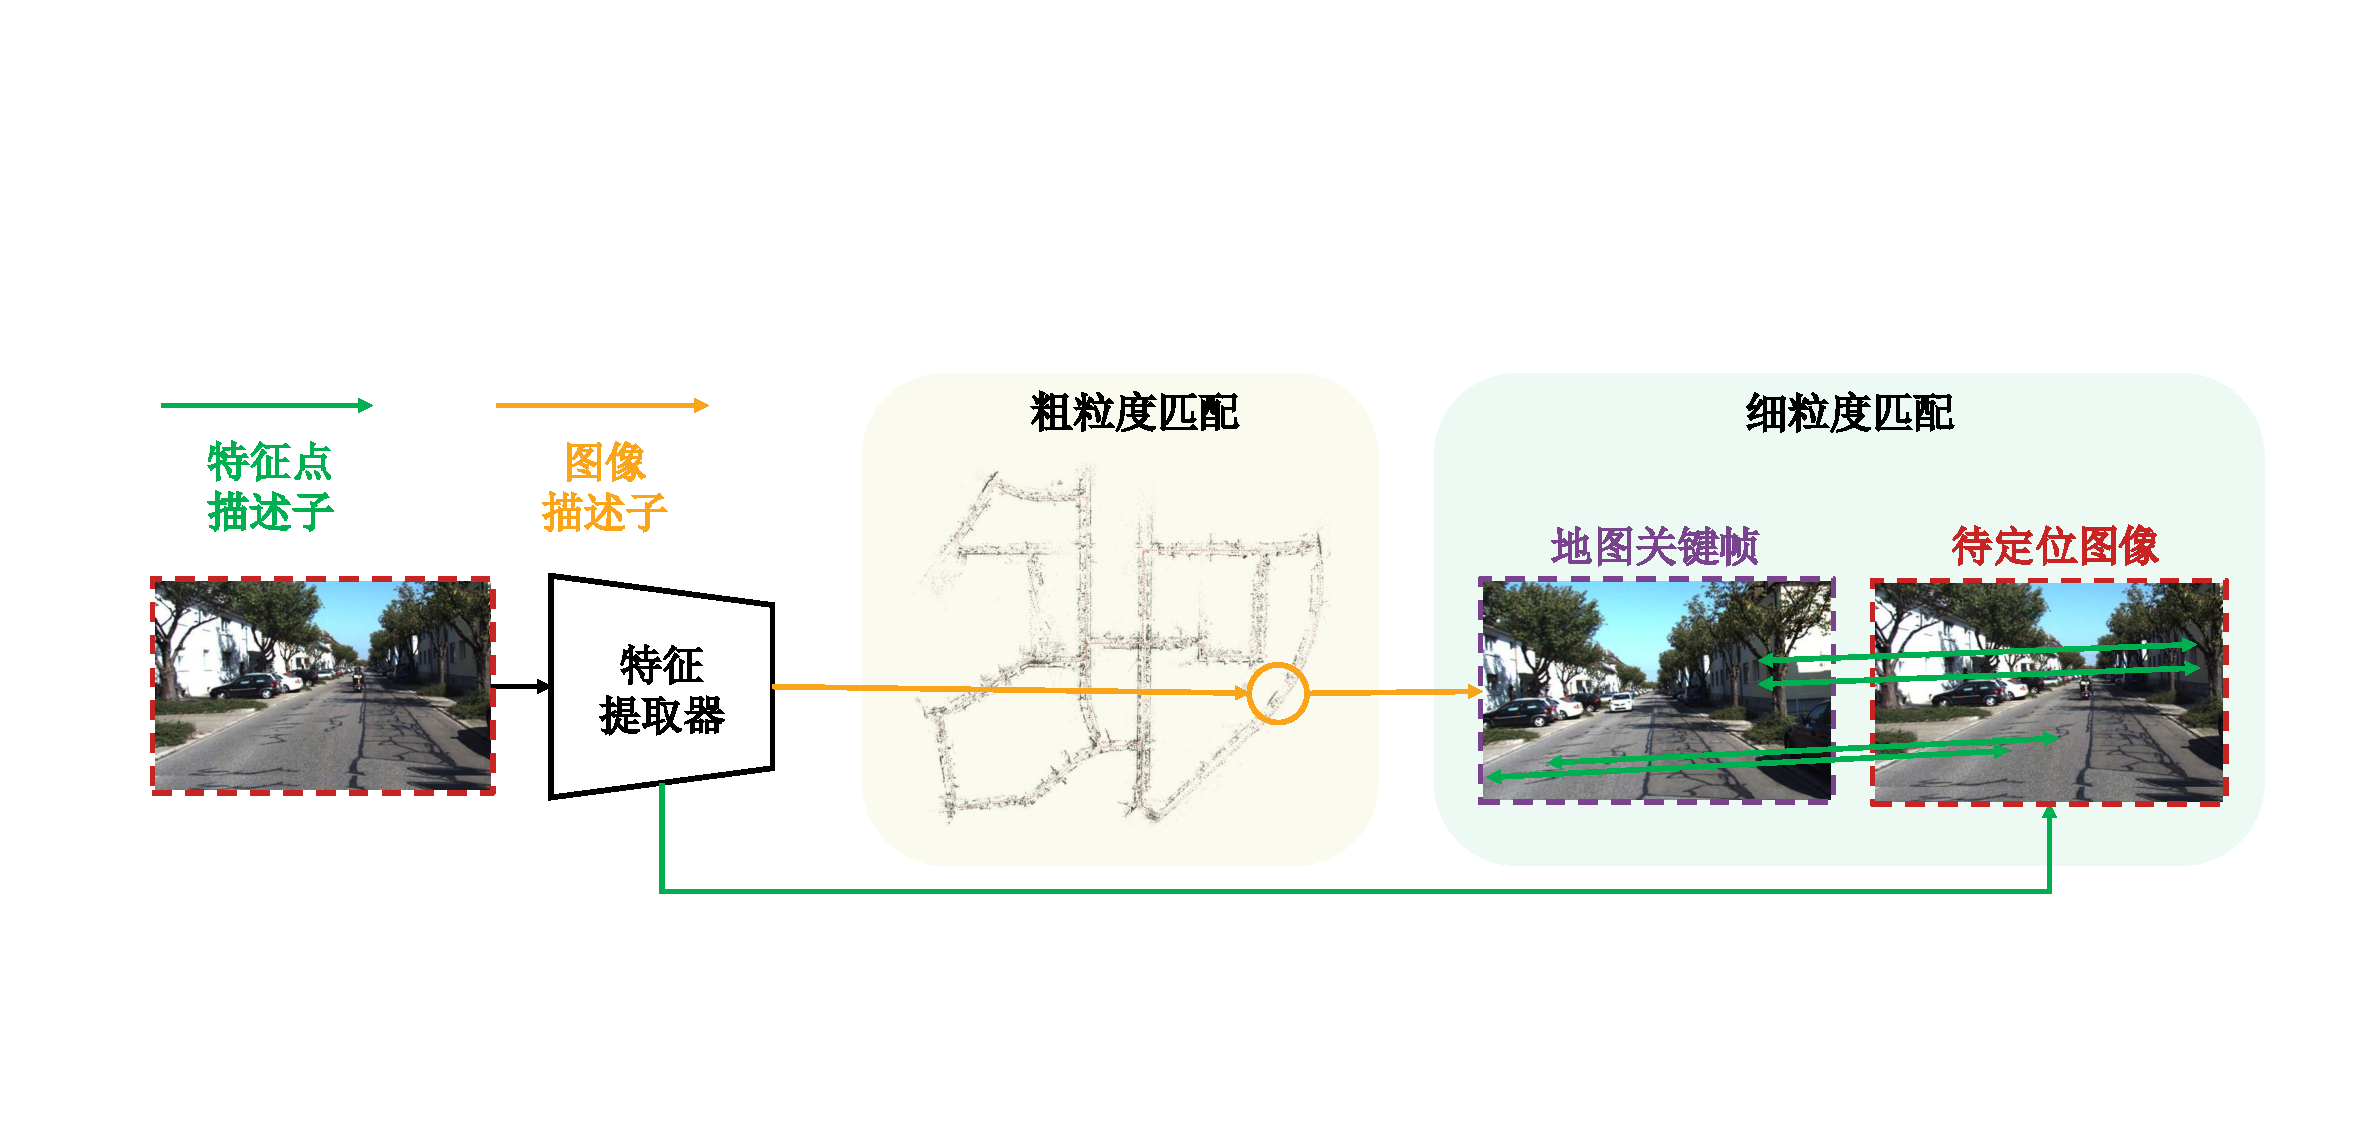
\includegraphics[width=1.0\linewidth]{matching.pdf}
  \caption{粗到细匹配过程}
  \label{fig:matching}
\end{figure}

如图~\ref{fig:matching} 所示,粗到细匹配过程首先从图像中提取图像描述子和特征点描述子。本文中的图像描述子使用NetVLAD\cite{arandjelovic2016netvlad}获取,这是一种基于CNN的图片特征提取网络,常被用来进行大规模的图像检索,证明其强大的特征判别能力,适合进行本文中的粗粒度匹配。本文中的特征点描述子使用Superpoint\cite{detone2018superpoint}获取,这是一种能够同时进行特征点提取和特征点描述子编码的神经网络,由于其经过了大量真实图片的训练,因此在真实场景下的表现依旧突出,适合本文的固定路线环境。

在提取了粗粒度和细粒度的特征描述子之后,还需要利用这两种粒度的描述子进行匹配。首先,粗匹配除了需要使用图像级别的粗粒度特征描述子以外,还需要使用一些位置先验信息。因为一段固定路线上可能会大量的关键帧,如果使用图像描述子对每一个关键帧都进行比对,会导致匹配效率较低,所以本文使用位置先验信息,将一部分距离过远的地图关键帧排除在匹配之外。这个位置先验信息可以通过以往的定位结果获得,如果处于定位开始阶段,没有可用的定位结果作为先验,那么可以使用全局坐标系下的原点为先验位置信息,这仍符合本文所探讨的国定路线定位场景。为了使粗粒度匹配能够为后续步骤提供充足的信息,匹配结果往往并不会只包含一个地图关键帧,本文选择一次匹配$N_c$个候选地图关键帧给后续步骤判断、使用。

细粒度匹配相较于粗粒度匹配过程更加直接,只需要将粗匹配的地图关键帧中的特征点及其描述子与当前图像的特征点及其描述子直接匹配即可。由于提取的特征点及其描述子都是基于深度神经网络的,因此匹配过程也选择基于深度神经网络的SuperGlue\cite{sarlin2020superglue}方法,其输入为特征点坐标和描述子,输出为它们之间的匹配关系。一旦新图像的特征点与地图关键帧的特征点匹配完成,细匹配即结束。

粗到细匹配过程在图像与地图关键帧之间建立了联系,这方便了将相机位姿的计算与全局坐标系对齐。在离线建图阶段,地图关键帧中的点已经与全局坐标系对齐,而新图像匹配的地图关键帧特征点也可以被赋予其对应的空间坐标,令这些点的空间坐标表示为$\{\symbf{p}_m^g \mid m \in \mathcal{M}\}$,其在新图像中对应的匹配点像素坐标观测为$\{\hat{\symbf{x}}_m \mid m \in \mathcal{M}\}$,其中 $\mathcal{M}$ 表示匹配关系。则新的位姿 $\symbf{T}^{c}_g$ 可通过求解以下投影优化问题获得:
\begin{equation}
  {\symbf{T}^{c}_g}^* = \text{arg} \min_{\symbf{T}_{c}^g} \sum_{m \in \mathcal{M}} \left( \Vert \hat{\symbf{x}}_m - \pi(\symbf{T}^{c}_g, \symbf{p}_m^g) \Vert^2_2 \right),
\end{equation}
若干现有方法 \cite{lepetit2009ep, gao2003complete} 可用于求解最优位姿 $\symbf{T}^{c}_g$,本课题采用EPnP(Efficient Perspective-n-Point)方法 \cite{lepetit2009ep}来高效地计算位姿,其最少仅需要4对匹配点即可完成计算。

此外,由于粗到细的匹配结果会给出$N_c$个候选地图关键帧,所以可以获得$N_c$个位姿估计结果$\{ \symbf{T}^{c}_{g,j} \}^{N_c}_{j=1}$(其中可能存在因为匹配点过少而匹配失败的情况),这些结果可以通过投票机制来获得较为鲁棒的位姿估计结果,具体过程如算法~\ref{alg2} 所示,其中的$\text{relang}(\cdot, \cdot),\text{relpos}(\cdot, \cdot)$分别表示计算两个转换矩阵的相对旋转角度和相对位移,相对角度和相对位移阈值分别设置为$t_r$和$t_p$,其具体取值参考表~\ref{tab:hyperparameters}。

\renewcommand{\algorithmicrequire}{\textbf{输入:}\unskip}
\renewcommand{\algorithmicensure}{\textbf{输出:}\unskip}
\begin{algorithm}
  \caption{Vote for visual localization result}
  \label{alg2}
  \small
  \begin{algorithmic}[1]
    \REQUIRE EPnP估计结果序列$Ts$,EPnP估计成功标志序列$Bs$,相对角度阈值$t_r$,相似位移阈值$t_p$
    \ENSURE 最优位姿估计结果$T_{r}$

    \STATE $T_{r} \leftarrow \symbf{I}_4$
    \STATE ${match}_{max} \leftarrow 0$
    \STATE $i \leftarrow 0$

    \WHILE{$i < \text{len}(Ts)$}
      \STATE $match \leftarrow 0$
      \IF{$Bs[i]$ indicates success}
        \STATE $j \leftarrow 0$
        \WHILE{$j < \text{len}(Ts) \land j \not= i$}
          \STATE $r \leftarrow \text{relang}(Ts[i], Ts[j])$
          \STATE $p \leftarrow \text{relpos}(Ts[i], Ts[j])$
          \IF{$r < t_r \land p < t_p $}
            \STATE $match \leftarrow match + 1$
          \ENDIF
        \ENDWHILE
        \IF{$match > {match}_{max}$}
          \STATE $T_{r} \leftarrow Ts[i]$
        \ENDIF
      \ENDIF
    \ENDWHILE
  \end{algorithmic}
\end{algorithm}

\section{转换矩阵初始化}

大多数情况下,粗到细定位是一种较为可信的定位信息来源,但是由于真实场景和建图场景可能存在较大差异,以及匹配等过程中的误差,所以仅使用粗到细定位的结果对于高精度要求的场景仍然是不足的。此外,每次粗到细定位的结果是相对独立的,因此其连续的定位结果也可能会存在跳变,如图~\ref{fig:zigzag} 所示,其中图的左侧是整个轨迹示意图,红色框选中局部区域,右侧是该区域详细展示。

\begin{figure}
  \centering
  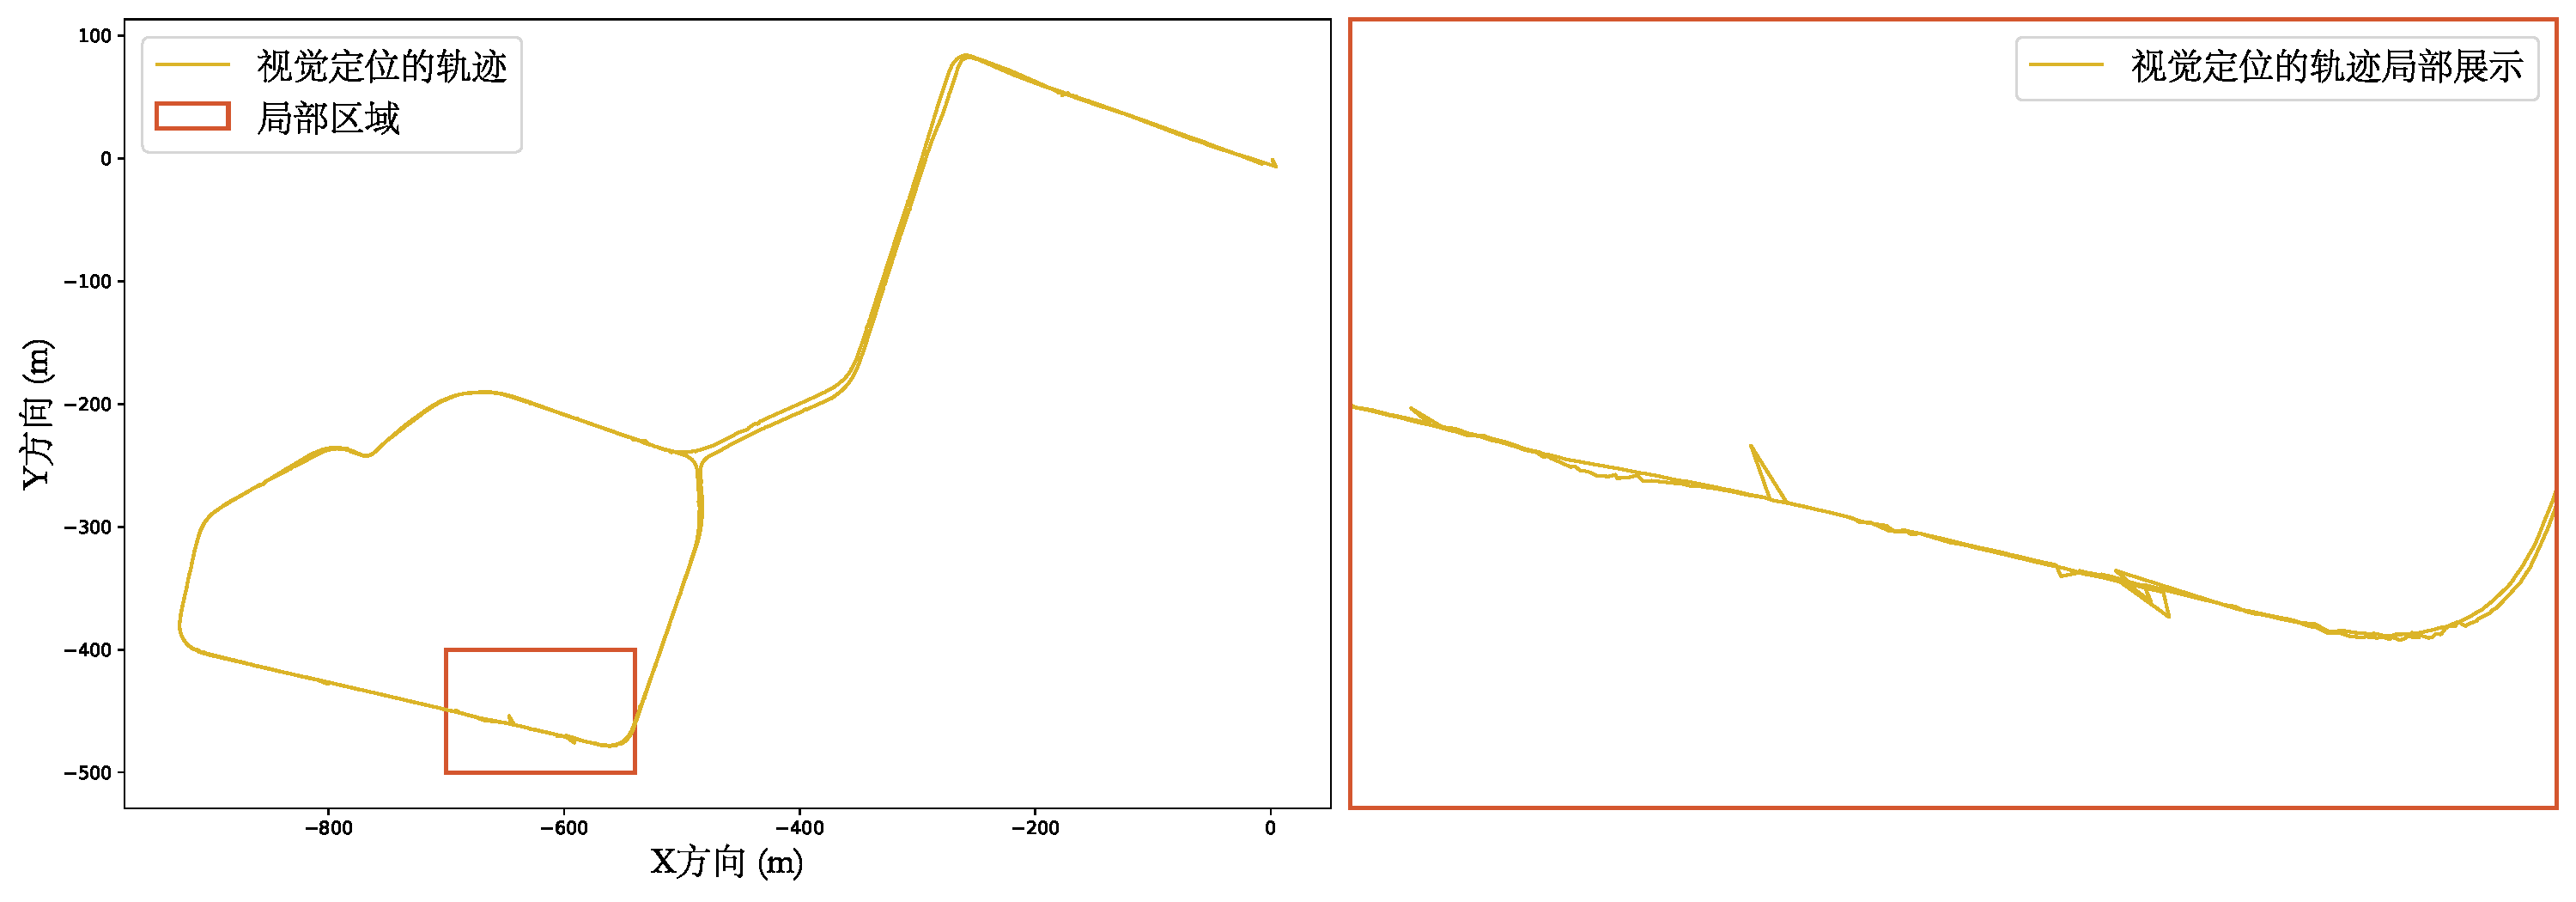
\includegraphics[width=1.0\linewidth]{zigzag.pdf}
  \caption{独立粗到细定位结果中的跳变}
  \label{fig:zigzag}
\end{figure}

为了解决这种跳变,增加最终定位结果的平滑性,需要使用视觉惯性里程计的相对位姿估计。除此之外,在粗到细定位偶尔失败的时候,还可以使用视觉惯性里程计的定位结果作为预备,能有效防止系统的整体崩溃。但是视觉惯性里程计和粗到细定位的坐标系并不一致,想要使用视觉惯性里程计的结果,需要将其转换到全局坐标系中。因此,需要一个转换矩阵初始化过程来获得两个坐标系的对齐参数,即转换矩阵$\symbf{T}_o^{g}$。对于每个相机$c_i$,其存在一个粗到细定位结果$\hat{\symbf{T}}^{g}_{c_i}$,还有一个视觉惯性里程计的定位结果$\hat{\symbf{T}}_{o}^{c_i}$,那么定位VIO世界坐标系与全局坐标系之间的变换为:
\begin{equation}
    \hat{\symbf{T}}_{o,i}^g = {\hat{\symbf{T}}^{g}_{c_i}} \hat{\symbf{T}}_{o}^{c_i}
\end{equation}
其中,${\hat{(\cdot)}}$表示带噪测量值。为了确定一个鲁棒的初始化变换$\symbf{T}_{o}^g$,本文使用了类似\ref{alg2} 的投票类算法,从前20个关键帧中收集的所有$\hat{\symbf{T}}_{o,i}^g$ 进行评估,选择内点样本数量最多的变换,该变换随后被用作对齐参数,将VIO获得的位姿映射到全局坐标系中。内点的选择同样使用相对角度和相对位移阈值$t_r,t_p$来进行判断,取值等同于\ref{sec:c2f_loc} 节中的同名变量。

由于转换矩阵相当于VIO世界坐标系和全局坐标系之间的对齐参数,所以其成功对齐对于整个定位系统的有效性至关重要。因此,只有当粗到细定位成功时,才会进入后续阶段,否则,将会使用滑窗形式不断丢弃旧的帧,更新最新的候选对齐参数,重新进行投票算法来估计$\symbf{T}_o^{g}$。

\section{有效性验证}
\label{sec:valid}
虽然粗到细定位使用了基于深度神经网络的特征提取和匹配方法来获得相对准确的地图点和当前观测之间联系,并使用基于投票的方式来鲁棒得获得新图像在全局坐标系中的粗略位姿$\symbf{T}_{c}^g$,但粗匹配和细匹配仍可能存在错误,因此定位观测的误差仍存在不确定性。虽然较小的误差可以通过后端优化来消除,但是如果出现了较大的突变,则可能对系统的稳定性产生严重的负面影响。因此,需要一个有效性验证过程来判断粗到细定位结果的可信度。

对于第$i$时刻的粗到细定位位姿测量值 ${\hat{\symbf{T}}^{g}_{c_i}}$,首先将其与第$i-1$时刻已经优化的位姿${\symbf{T}}^{g}_{c_{i-1}}$进行比较,如果满足以下条件,则认为新粗到细定位测量值是有效的:
\begin{equation}
\label{eq:check}
\begin{cases}
    [\hat{\symbf{T}}_{o}^{c_{i-1}}\hat{\symbf{T}}^{o}_{c_i}]_{t} - [\symbf{T}_{g}^{c_{i-1}}\hat{\symbf{T}}^{g}_{c_i}]_{t} < \lambda_{d}, \\
    [\hat{\symbf{T}}^{c_i}_o \hat{\symbf{T}}_{c_{i-1}}^o \symbf{T}^{c_{i-1}}_g \hat{\symbf{T}}_{c_{i}}^g]_{d} < \lambda_{r},
\end{cases}
\end{equation}
其中,$[\cdot]_{t}$ 表示提取变换矩阵的平移分量,$[\cdot]_{d}$ 表示提取变换矩阵的旋转角度:首先将变换矩阵的旋转部分提出,然后通过罗德里格斯旋转公式获取相对旋转角度。阈值 $\lambda_{t}$ 和 $\lambda_{d}$ 分别是判断新粗到细定位观测的相对平移和相对旋转角度是否符合有效性的条件阈值,具体取值参考\ref{tab:hyperparameters}。

如果粗到细定位的位姿测量值未能满足条件 \eqref{eq:check},则被视为不可接受,在这种情况下,使用从VIO转换得到的测量值
\begin{equation}
    \hat{\symbf{T}}_{g}^{c_i} = \symbf{T}_{o}^g \hat{\symbf{T}}_{o}^{c_i}
\end{equation}
作为优化的初始位姿。

\section{紧耦合优化}
\label{sec:tight_opt}
粗到细定位和视觉惯性里程计的定位测量结果都无法单独达到较高的精度:粗到细定位的测量值由于与先验地图的匹配误差而存在噪声,而VIO的测量值则受到累积漂移的影响。因此,融合这两种测量值的优化方法对最终精度至关重要。本文提出使用与先验地图紧耦合的位姿图来优化最终位姿。紧耦合指的是优化过程中,相机位姿的优化与和地图点云结构的优化同时进行。在这种优化模式下,地图的先验地图结构不再是固定不变的,而转化为一种概率地图,基于这种概率地图,后段的位姿优化也从最大似然估计转化为一种最大后验概率估计。这样做的优势是将点云结构的不确定性考虑到优化过程中,从而提高了优化的鲁棒性。

如果当前已有的相机帧观测到的点结构表示为 $\mathcal{P} = \{\symbf{p}^g_m | m = 1, \dots, M\}$,它们的观测表示为 $\mathcal{X} = \{\hat{\symbf{x}}_{im}|i=1,\dots, N\}$,其中 $\symbf{x}_{im}$ 表示 $i$-th 相机帧对点 $\symbf{p}^g_m$ 的观测,则位姿估计过程可以表示为最大化概率:
\begin{equation}
\label{eq:prob}
  \max_{\mathcal{T}, \mathcal{P}} p(\mathcal{T}, \mathcal{P} | \mathcal{X}),
\end{equation}
其中,$\mathcal{T} = \{ \symbf{T}_{c_i}^g | i=1,\dots, N\}$表示位姿的集合。又因为:
\begin{equation}
p(\mathcal{T}, \mathcal{P} | \mathcal{X}) \propto p(\mathcal{X} | \mathcal{T}, \mathcal{P}) \cdot p(\mathcal{T}, \mathcal{P}),
\end{equation}
即概率~\eqref{eq:prob}所表示的最大后验概率可以分解为似然和先验的乘积。其中,$p(\mathcal{X} | \mathcal{T}, \mathcal{P})$ 表示似然,$p(\mathcal{T}, \mathcal{P})$ 表示先验。假设位姿和点结构的先验分布相互独立,可以将先验分解为:
\begin{equation}
  p(\mathcal{T}, \mathcal{P}) = p(\mathcal{T}) \cdot p(\mathcal{P}).
\end{equation}
由于我们主要关注点结构的先验,可以将后验分布重写为:
\begin{equation}
\begin{aligned}
  p(\mathcal{T}, \mathcal{P} | \mathcal{X}) &\propto p(\mathcal{X} | \mathcal{T}, \mathcal{P}) \cdot p(\mathcal{T}) \cdot p(\mathcal{P}) \\
  &\propto p(\mathcal{X} | \mathcal{T}, \mathcal{P}) \cdot p(\mathcal{P}).
\end{aligned}
\end{equation}
因此,位姿和点结构的估计可以表示为:
\begin{equation}
  \label{eq:max_post}
  \mathcal{T}^*, \mathcal{P}^* = \underset{\mathcal{T}, \mathcal{P}}{\text{arg max}} \left[ p(\mathcal{X} | \mathcal{T}, \mathcal{P}) \cdot p(\mathcal{P}) \right],
\end{equation}
其中各项展开为:
\begin{equation}
p(\mathcal{X} | \mathcal{T}, \mathcal{P}) = \prod_i \prod_m p(\symbf{x}_{im} | \symbf{T}_g^{c_i}, \symbf{p}_m^g),
\end{equation}
\begin{equation}
p(\mathcal{P}) = \prod_m p(\symbf{p}_m^g).
\end{equation}
假设似然和先验均为高斯误差,则两个概率可以表示为:
\begin{equation}
  p(\symbf{x}_{im} | \symbf{T}_g^{c_i}, \symbf{p}_m^g) = \frac{1}{2\pi\sqrt{|\symbf{\Sigma}_{im}|}}e^{-\frac{1}{2}\symbf{r}_{im}^T \cdot {\symbf{\Sigma}_{im}}^{-1}\cdot \symbf{r}_{im}}
\end{equation}
\begin{equation}
  p(\symbf{p}_m^g) = \frac{1}{\sqrt{(2\pi)^3|\symbf{\Sigma}_m|}}e^{-\frac{1}{2}\symbf{r}_{m}^T \cdot {\symbf{\Sigma}_{m}}^{-1} \cdot \symbf{r}_{m}}
\end{equation}
其中$\symbf{\Sigma}_{im}\in \mathbb{R}^{2\times 2}$表示视觉观测的误差的协方差矩阵,$\symbf{\Sigma}_{m} \in \mathbb{R}^{3 \times 3}$表示地图点的先验误差的协方差矩阵,$\symbf{r}_{im}$和$\symbf{r}_m$分别为视觉观测误差和地图点云先验误差,其定义在后文详细介绍。因此式~\eqref{eq:max_post}的概率取负对数并省略常量值可重写为:
\begin{equation}
\label{eq:min_logprob}
\mathcal{T}^*, \mathcal{P}^* = \underset{\mathcal{T}, \mathcal{P}}{\text{arg min}} \left( \sum_i \sum_m \| \symbf{r}_{im} \|_{\symbf{\Sigma}_{im}}^2 + \sum_m \| \symbf{r}_m \|_{\symbf{\Sigma}_{m}}^2 \right).
\end{equation}
至此,已经将求解概率最大化问题转化为优化非线性残差问题。其中,$\symbf{r}_{m}$表示的先验约束是本文区别于一般定位建图方法的关键点:经典的位姿优化将地图点云结构视为固定不变的参数,而本文将地图点云结构建模为以点云三维坐标为中心的高斯概率分布。在这种建模下,点云的空间坐标也作为待优化的参数。这种基于地图点的先验值进行优化的方式,也可以看作是一种最大后验概率(Maximum A Posteriori Probability, MAP)优化。

式~\eqref{eq:min_logprob}是一个非线性优化问题,可以通过优化位姿图的形式进行优化。位姿图是一种表示优化变量及其相互关系的图数据结构,其将优化问题转化为一个图,图中的节点表示待优化的参数,边表示约束,通过最小化边上的残差来求解最优参数。因此,如果要求解位姿$\{ \symbf{T}_{c_i}^g | i=1,\dots, N\}$和地图点云结构$\{\symbf{p}^g_m | m = 1, \dots, M\}$,可以将其视作图优化的顶点,而残差$\symbf{r}_{im}, \symbf{r}_m$可以作为图的边,此处定义其为地图观测边和地图点先验边。

\begin{figure}
  \centering
  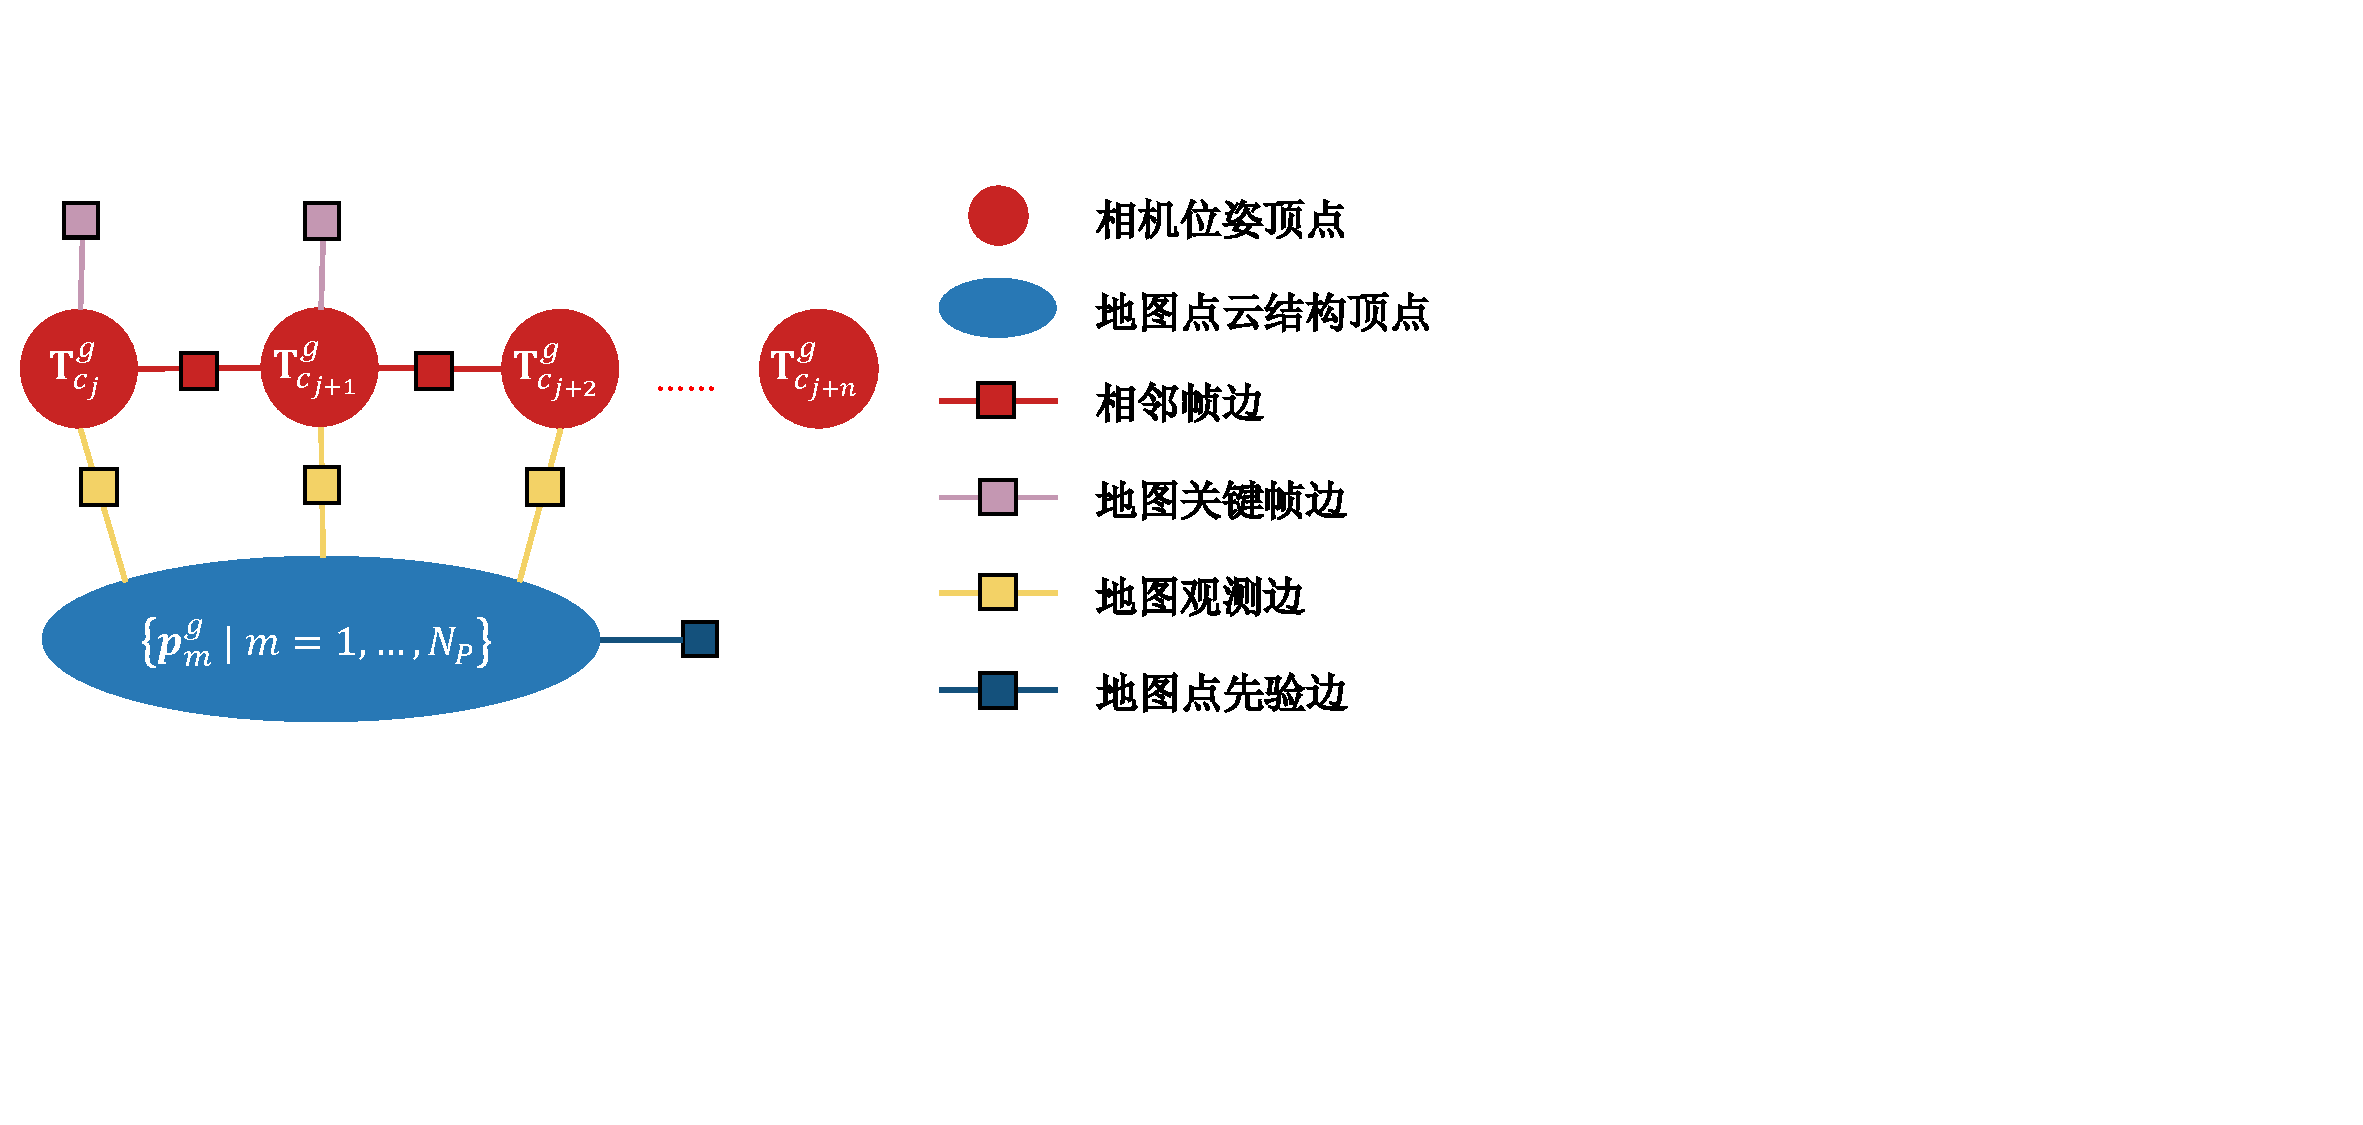
\includegraphics[width=1.0\linewidth]{graph.pdf}
  \caption{紧耦合优化位姿图}
  \label{fig:graph}
\end{figure}

除了上述两种残差,根据视觉惯性里程计和粗到细定位给出的位置观测,还可以构造相邻帧边和地图关键帧边,整个紧耦合优化位姿图如图~\ref{fig:graph} 所示。首先已经定义的地图观测边$\symbf{r}_{im}$可以表示为:
\begin{equation}
  \symbf{r}_{im} = \hat{\symbf{x}}_{im} - \pi(\symbf{T}_{c_{i}}^g, \symbf{p}^g_m),
\end{equation}
其中,$\hat{\symbf{x}}_{im}$是地图点$\symbf{p}^g_m$在相机位姿$\symbf{T}_{c_{i}}^g$下的视觉观测值。地图点先验边$\symbf{r}_m$可以表示为:
\begin{equation}
  \symbf{r}_{im} = \hat{\symbf{x}}_{im} - \pi(\symbf{T}_{c_{i}}^g, \symbf{p}^g_m),
\end{equation}
其中,$\hat{\symbf{p}}^g_m$是点$\symbf{p}^g_m$的先验位置,在建图阶段即确立。

相邻边用于约束位姿的平滑性,其表达式为:
\begin{equation}
    \symbf{r}_i = [(\hat{\symbf{T}}^{c_i}_{o} \hat{\symbf{T}}^{o}_{c_{i+1}})^{-1} (\symbf{T}^{c_{i}}_g \symbf{T}_{c_{i+1}}^g)]_{lie},
\end{equation}
其中,$\hat{\symbf{T}}^{c_i}_{o}$ 是视觉惯性里程计的测量值,$[\cdot]_{lie}$ 表示求解矩阵的李代数(Lie algebra)\cite{bourbaki1989lie}。虽然视觉惯性里程计在运行一段时间后会产生世界坐标系的漂移,但是其获得的帧间相对运动还是相对准确的,因此可以用于约束相邻帧的位姿。

如果位姿图中存在由粗到细定位初始化的相机位姿,则必定存与之相对应的参考地图关键帧。假设相机位姿$\symbf{T}_{c_{i}}^g$对应于地图关键帧$\symbf{T}_{k_{j}}^g$,则地图关键帧边可以构造为:
\begin{equation}
    \symbf{r}_{ij} = [(\hat{\symbf{T}}^{k_j}_{c_{i}})^{-1} (\symbf{T}^{k_{j}}_g \symbf{T}_{c_{i}}^g)]_{lie},
\end{equation}
其中,$\hat{\symbf{T}}^{k_j}_{c_{i}}$是使用地图关键帧和当前图像计算得到的地图定位测量值。

最终,所有需要优化的残差结合起来可以作为整体优化目标:
\begin{equation}
\begin{aligned}
  \mathcal{J} = & \sum_{i,i+1\in\mathcal{S}}\|\symbf{r}_i\|_{\symbf{\Sigma}_{i}}^2 + \sum_{i,j\in\mathcal{C}}\rho(\|\symbf{r}_{ij}\|_{\symbf{\Sigma}_{ij}}^2) \\ 
  &+ \sum_i \sum_m \rho(\| \symbf{r}_{im} \|_{\symbf{\Sigma}_{im}}^2) + \sum_m \rho(\| \symbf{r}_m \|_{\symbf{\Sigma}_{m}}^2),
\end{aligned}
\end{equation}
其中,$\mathcal{S}$ 表示相邻帧的集合,$\mathcal{C}$ 表示有参考地图关键帧的位姿集合。协方差矩阵$\symbf{\Sigma}_{i},\symbf{\Sigma}_{ij},\symbf{\Sigma}_{im},\symbf{\Sigma}_{m}$一般作为超参数来平衡各种误差在数量级上的不平衡。因为在矩阵的李代数中有部分表示旋转误差,部分表示平移误差,旋转误差的模等于转动角,这个值一般较小,而平移误差的模一般表示位移距离,这个值一般较大,所以设置
\begin{equation}
  \symbf{\Sigma}_{i} = \symbf{\Sigma}_{ij} = 
  \begin{bmatrix}
    0.1 \cdot \symbf{I}_3 & \symbf{0}_{3\times 3} \\
    \symbf{0}_{3\times 3} & 0.01 \cdot \symbf{I}_3
  \end{bmatrix},
\end{equation}
其中$\symbf{I}_3$表示3维的单位矩阵,$\symbf{0}_3$表示3维的零矩阵。$\symbf{\Sigma}_{im}$一般表示相机的观测协方差,这个值一般根据相机的焦距$f$而确定,本文设置为
\begin{equation}
  \symbf{\Sigma}_{im} = \frac{1}{f} \cdot \symbf{I}_2.
\end{equation}
最后,对于地图点的先验协方差,此处根据其建图的像素误差确定
\begin{equation}
  \symbf{\Sigma}_{m} = \text{diag}({\symbf{R}_{jm}^g}^{-1}\cdot\symbf{K}^{-1}\cdot z_m \cdot u_m \cdot \symbf{I}_3 - {\symbf{R}_{jm}^g}^{-1}\cdot\symbf{t}_{jm}^g),
\end{equation}
其中$\text{diag}(\cdot)$表示将向量作为对角线元素构造对角矩阵,$\symbf{R}_{jm}^g$和$\symbf{t}_{jm}^g$分别表示观测到地图点$\symbf{p}_m^g$最大误差的地图关键帧在全局坐标系下的旋转矩阵和平移向量,$\symbf{K}$表示相机的内参矩阵,$z_m$和$u_m$分别表示地图点的深度和像素误差,深度根据旋转和平移计算,像素误差值在建图阶段记录。

除此之外,为了约束优化的规模,提升系统的实时性,本文使用滑动窗口的方法来保证只有定量的位姿参与优化,即确定$\mathcal{T} = \{ \symbf{T}_{c_i}^g | i=1,\dots, N\}$中的$N$是一个合理值。另外针对每一帧的地图点优化数量,本文选择只将单帧所能观测到的地图点按照重投影误差排序,只选择其中的前$\kappa$个点进入位姿图优化,保证了点云结构$\mathcal{P} = \{\symbf{p}^g_m | m = 1, \dots, M\}$的优化规模
\begin{equation}
  M \le \kappa \cdot N.
\end{equation}

\section{转换矩阵更新}

转换矩阵控制着从VIO世界坐标系到全局坐标系的转换,而在某些情况,例如粗到细定位偶然失效时,其关系着视觉惯性里程计的结果能否被紧耦合优化正确初始化,所以有必要对其进行实时维护。由于视觉惯性里程计本身存在的漂移累积,所以在运行一段时间之后,转换矩阵必然会出现无法将VIO世界坐标系和全局坐标系对齐的情况。因此,需要一个实时的转换矩阵更新过程来保证定位的准确性。

在本文中,更新矩阵的实时维护就由转换矩阵更新步骤来完成。其主要工作是在每次紧耦合优化完成之后,根据优化结果更新转换矩阵。假设优化后的相机位姿为$\{ \symbf{T}_{c_i}^g | i=1,\dots, N\}$,则可以计算出当前每个相机的转换矩阵$\{ \hat{\symbf{T}}_{o,i}^g | i=1,\dots, N\}$,假设待更新的转换矩阵为$\check{\symbf{T}}_{o,i}^g$,则更新算法如算法~\ref{alg3} 所示。
\renewcommand{\algorithmicrequire}{\textbf{输入:}\unskip}
\renewcommand{\algorithmicensure}{\textbf{输出:}\unskip}
\begin{algorithm}
  \caption{Update the transformation matrix}
  \label{alg3}
  \small
  \begin{algorithmic}[1]
    \REQUIRE 旧转换矩阵$T_{old}$,当前相机的转换矩阵序列$Ts$
    \ENSURE 新转换矩阵序列$T_{new}$

    \STATE $acc_{inlier} \leftarrow 0$
    \STATE $T_{new} \leftarrow T_{old}$

    \FOR{$T$ in $Ts$}
      \STATE $r \leftarrow \text{relang}(T_{old}, T)$
      \IF{$r < 60\degree$}
        \STATE $acc_{inlier} \leftarrow acc_{inlier} + 1$
      \ENDIF
    \ENDFOR

    \IF{$acc_{inlier} \ge 0.5 \cdot \text{len}(Ts)$}
      \STATE $R_{acc} \leftarrow \symbf{I}_3$
      \STATE $t_{acc} \leftarrow \symbf{0}_3$
      \FOR{$T$ in $Ts$}
        \STATE $R,t \leftarrow \text{decompose}(T)$
        \STATE $R_{acc} \leftarrow R_{acc} + R$
        \STATE $t_{acc} \leftarrow t_{acc} + t$
      \ENDFOR
      \STATE $U, \Sigma, V = \text{SVD}(R_{acc})$
      \STATE $R_{new} \leftarrow U\cdot \text{transpose}(V)$
      \STATE $t_{new} \leftarrow \frac{1}{\text{len}(Ts)}\cdot t_{acc}$
      \STATE $T_{new} \leftarrow \text{compose}(R_{new}, t_{new})$
    \ENDIF
  \end{algorithmic}
\end{algorithm}

算法中$\text{decompose}(\cdot)$表示将转换矩阵分解为旋卷矩阵和位移向量,$\text{compose}(\cdot, \cdot)$则表示将旋卷矩阵和位移向量组合为转换矩阵,$\text{SVD}(\cdot)$表示奇异值分解函数,$\text{tranpose}(\cdot)$表示矩阵转置操作。

\section{本章总结}
本章主要介绍了紧耦合地图定位模块的设计,其输入包括当前的图片、先验地图信息以及视觉惯性里程计,其主要工作就是使用前面工作的信息综合估计当前相机的位置和姿态。首先,本章介绍了粗到细定位的设计,其主要工作是使用深度神经网络提取特征,然后使用基于投票的方法估计相机的位置和姿态。接着,本章介绍了转换矩阵初始化和有效性验证的设计,这两部配合工作可以确保有一个正确的初始化位姿可以被紧耦合优化使用。然后,本章介绍了紧耦合优化的设计,其主要工作是将粗到细定位和视觉惯性里程计的结果融合,然后使用图优化的方法估计相机的位置和姿态。最后,本章介绍了转换矩阵更新的设计,其主要工作是根据优化后的结果更新转换矩阵。